\documentclass[hidelinks, 12pt, oneside]{article}
\usepackage{bookmark}
\usepackage{graphicx}
\usepackage{hyperref}
\usepackage{titlesec}
\setcounter{secnumdepth}{4}
\usepackage[utf8]{inputenc}
\usepackage[english]{babel}


\begin{document}
	
	\begin{center}
    \centering
    
%University logo
    
\includegraphics[width=144px]{img/icon.png}
    \rule{0\linewidth}{0.15\linewidth}\par
    
    		\begin{center}
		{\uppercase{\Large User Manual\par}}
   		{\Large iCrawler \par}
   			\vspace{1cm} 
   		{\Large Emilio Mumba  \par} 
    		\vspace{1cm}
		   		
    		{\Large The 5 Concurrent Nodes \par} 
    		\vspace{1cm}
		
		{\normalsize Khathutshelo Shaun Matidza\par}
		{\normalsize Sylvester Sandile Mpangane\par}
		{\normalsize Thabang Michael Letageng\par}
		{\normalsize Matthew Nel\par}
		
		\end{center}

		\textbf{}		
		\centering
		\vspace{2cm}
		Department of Computer Science, University of Pretoria

		
	 	{\Large  September 2015}
\end{center}
\clearpage


	\tableofcontents
	\newpage
	
	\section{Overview}
	\begin{flushleft}
		This document is intended to serve as a reference for the development methodology used for the iCrawler App; which was proposed 
	by Emilio Mumba for COS301 final year project.\newline\newline
	The app is intended to promote readiness in digital forensics, protect users from malicious entities and activities, and provide proactive 
	measures that are undertaking by the mobile device user/owner. It monitors the user's activities and collects data/logs from the device. The data
	is then reported to a desktop computer which generates reports that give the investigator (parent/guardian/employer) a good starting point in his/her investigation.\newpage
	\end{flushleft}

	
	\section{Roles}
	There are three core roles[10] with a range of ancillary roles. These core roles are committed to the project in the scrum process.
	\subsection{Product Owner}
	\textbf{Name:} Emilio Raymond Mumba\newline
	\textbf{Responsibilities:} He is responsible for product vision; he accepts or rejects each product increment. He constantly re-prioritizes the Product Backlog, adjusting any longterm expectations such as release plans. He is the final arbiter of requirements questions.
 	\subsection{Development Team}
 	\textbf{Name:} The 5 Concurrent Nodes\newline
	\textbf{Responsibilities:} Intensely collaborative and cross-functional. They are responsible for delivering potentially shippable increments (PSIs) of product at the end of each sprint (the sprint goal). 
	The team
	is made up of four individuals who do the actual work.
	\subsection{Scrum Master}
 	\textbf{Name:} Khathutshelo Shaun Matidza\newline
	\textbf{Responsibilities:} He is responsible for ensuring that the team follows the agreed scrum processes, facilitating key sessions, and encourages 
	the team to improve. He enforces timeboxes. He is part of the development team\newpage
	
	\section{Events}
	\subsection{Sprint}
	A sprint is the basic unit of development in scrum. It is restricted to a specific duration. The duration is fixed in advance for each sprint and is 
	normally between one week and one month, with two weeks being the most common.\newline\newline
	At the beginning of a sprint we hold a \emph{sprint planning event}. This event takes place after every contact session with the client or module coordinators,
	which is usually every two weeks. During this planning we decide on what work needs to be done during the sprint duration. Our client (stakeholder) has access 
	to our Git Hub repository, which at the end of each sprint he gets to see the current progress of the app.\newline
	When the sprint comes to an end we hold a \emph{sprint review}. Here we review the work that was completed and the planned work that was not completed during the 
	past sprint. We also present the completed work to the client/stakeholders (a.k.a \emph{demo}).\newline
	The review is thus followed by a \emph{sprint retrospective}. On this event we reflect on the past sprint; we identify and agree on continuous process improvement actions. 
	\subsection{Daily Scrum}
 	We hold a \emph{daily scrum} (or stand-up) each day during a sprint to discuss what an individual did the day before, what they plan on doing today and also if they 
 	see any impediments that might prevent them from reaching the sprint goal. The best time we opted for is after a lecture that we all share; this is to try and have 
 	all members	to attend the daily scrum (although attendances of all members is not compulsory). The length of the daily scrum is constrained to 15min max., which explains 
 	why we stand.\newpage 
 	
 	\section{Artifacts}
 	\subsection{Product backlog}
 	The \emph{product backlog} comprises an ordered list of \emph{requirements} that a scrum team maintains for a product. It consists of features, bug fixes, non-functional 
 	requirements, etc.-whatever needs doing in order to successfully deliver a viable product.\newline\newline 	
 	\begin{tabular}{|p{6cm}|p{4cm}|p{3cm}|}
			\textbf{Item} & \textbf{Est. time} & \textbf{Priority}\\
			\hline
			User login & 5hrs & High\\
			\hline
			User register & 5hrs & High\\
			\hline
			Retrieve device info & 5hrs & High\\
			\hline
			Database & 20hrs & High\\
			\hline
			Retrieve installed apps info & 5hrs & Low\\
			\hline
			Run in background & 5hrs & High\\
			\hline
			Sms monitor & 5hrs & High\\
			\hline
			Browser monitor & 5hrs & High\\
			\hline
			Dashboard GUI & 15hrs & Medium\\
			\hline
			User manual & 30hrs & Medium\\
			\hline
			App GUI & 5hrs & Medium\\
			\hline
			Call monitor & 5hrs & High\\
			\hline
			Functional requirements & 5hrs & High\\
			\hline
			Architectural requirements & 5hrs & High\\
			\hline
			Password recovery & 5hrs & Medium\\
			\hline
			Data encryption & 5hrs & High\\
			\hline
			Local storage & 10hrs & Low\\
			\hline
			Splash screen & 10hrs & Medium\\
			\hline
			Data summary & 20hrs & High\\
			\hline
			Retrieve wifi activities & 6hrs & Low\\
			\hline
			App tour & 6hrs & Medium\\
			\hline
			Development methodology & 5hrs & High\\
			\hline
			Data usage & 6hrs & Low\\
			\hline
			&&\\
			\hline
		\end{tabular}\newpage
		
 	\subsection{Sprint backlog}
 	The \emph{sprint backlog} is the list of work the development must address during the next sprint.\newline\newline
 	\begin{tabular}{|p{6cm}|p{4cm}|p{3cm}|}
			\textbf{Item} & \textbf{Duration} & \textbf{Feedback}\\
			\hline
			App GUI & 3rd May - 15th May & Completed\\
			\hline
			User registration\newline Run in background\newline Functional requirements doc\newline Database & 17th May - 29th May & Completed\\
			\hline
			User login\newline Dashboard GUI\newline Retrieve device info\newline Sms monitor & 24th June - 24th July & Completed\\
			\hline
			Browser monitor\newline Calls monitor& 27th July - 7th Aug & Completed\\
			\hline
			Retrieve installed apps\newline Data summary & 9th Aug - 21 Aug & Completed\\
			\hline
			REST api\newline password recovery & 24th Aug - 4th Sept & Completed\\
			\hline
			User manual\newline app tour guide & 7th Sept - 2nd Oct & Completed\\
			\hline
			Retrieve wireless activity\newline Data encryption\newline Data usage & 6th Oct - 16th Oct & In progress\\
			\hline
			Splash screen\newline Development methodology doc\newline Architectural requirement doc &19th Oct - 23th Oct & Incomplete\\
			\hline
		\end{tabular}\newpage
 	\subsection{Product increment}
 	The \emph{increment} (or \emph{potentially shippable increment}, PSI) is the sum of all the product backlog items completed during a sprint and all previous sprints. At the end 
 	of a sprint, the increment must be completed, according to the team's Definition of Done (DoD), and in a usable condition regardless of whether the product owner decides to actually
 	release it.\newline
 	\href{https://github.com/u11241617/COS301-Mobile-Monitoring-App/}{\emph{Click here to go to gitHub repository}}\newline
 	\subsection{Sprint burn-down chart}
	The \emph{sprint burndown chart} is a public displayed chart showing remaining work in the sprint backlog. It gives a simple view of the sprint progress. During the sprint planning 
	the ideal burndown chart is plotted. During the sprint, each member picks up tasks from the sprint backlog and works on them. The burndown chart is updated day by day.\newline\newline
	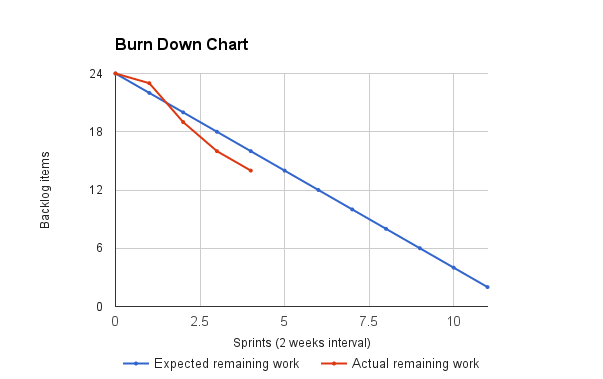
\includegraphics[width=400px]{img/burndown.png}\newline
	\href{https://docs.google.com/spreadsheets/u/3/d/1Qa7quxQTuZJmRNlt84Dl4iSXsZh-cYIeFgFJ_hzmv5k/edit?usp=drive_web}{\emph{Click here for online burn-down chart}}\newpage
 	
 	\section{Terminology}
 	The following explains some of the terms used in the scrum process.\newline\newline
 	\textbf{Scrum team}\newline
 	Product owner, scrum master and development team\newline\newline
 	\textbf{Product owner}\newline
 	The person responsible for maintaining the product backlog by representing the interests of the stakeholders, and ensuring the value of the work the development team does.\newline\newline
 	\textbf{Scrum master}\newline
 	The person responsible for the scrum process, making sure it is used correctly and maximizing its benefits.\newline\newline
 	\textbf{Development team}\newline
 	A cross-functional group of people responsible for delivering potentially shippable increments of product at the end of every sprint.\newline\newline
 	\textbf{Sprint burn-down chart}\newline
 	Daily progress for a sprint over the sprint's length.\newline\newline
 	\textbf{Product backlog}\newline
 	A prioritized list of high-level requirements.\newline\newline
 	\textbf{Sprint backlog}\newline
 	A prioritized list of tasks to be completed during the sprint.\newline\newline
 	\textbf{Sprint}\newline
 	A time period (typically 1-4 weeks) in which development occurs on a set of backlog items that the team has committed to.
 	
\end{document}